Our final goal was to determine file sizes for which file system adds another layer of indirection. Ext4 uses extents to manage data blocks. Extents are organized into a tree, where each extent can point either to another extents (interior extent) or to block group (leaf extent). Block group is a physically continuous range of blocks, where each block has 4096 bytes. Each block group can address up to $2^15$ continuos blocks, which is total of 128 MB. Each inode stores direct pointers to up to four leaf extents. When file size outgrows the four existing extents and filesystem creates fifth extent, it also creates a new metadata block. At that point, we say that filesystem adds one layer of indirection.

Let's consider three scenarios that might happen when we append one block to the file:
\begin{enumerate}
\item Last block group in the file is extended. In this case, we write data block and update one block group.
\item There is no more space left in the last block group. We need to create new block group and new extent.
\item There is no more space left in the last block group, and all four extents in the file inode are used. We need to create new block group, new extent and also reorganize four extents in the file inode.
\end{enumerate}

The assumption we need to make to be able to detect these events is that case 3 is considerably slower than 2 and case 2 is considerably slower than 1. We also need to assume that any other slowdown that might happen during the process of writing bytes is uncorrelated with file size and will be eliminated by only taking into account lower bound of multiple runs.

Group blocks in ext4 can be arbitrarily sized and depend on disk layout. If a block following the group block is used, we need to create a new group block. If it's free, we would just extend the group block. Because of this, our hypothesis is that the moment when ext4 adds another layer of indirection doesn't depend only on file size, but also on disk layout and other factors.

We propose the experiment presented in Figure \ref{fig:p4pseudo} to verify our hypothesis. By timing one-byte append, we should be able to distinguish between the three different events mentioned earlier. We run the experiment five times and take the minimum latency for each data point. If our hypothesis holds and adding layer of indirection does not depend only on file size, we expect to see the flat line as a result of our experiment. This result would also prove our hypothesis, showing there is no single file size where append needs to take more time to create new metadata blocks.

\begin{figure}
\begin{algorithmic}
\STATE create a $file$
\STATE $buffer\_size \leftarrow$ 4096
\FOR{$i = 0$ to $MAX\_SIZE$}
\STATE $buffer \leftarrow$ random $buffer\_size$ bytes
\STATE open a file with O\_SYNC flag, seek to the end
\STATE start\_timer
\STATE write first byte of $buffer$
\STATE end\_timer and save the result
\STATE write the rest $buffer\_size - 1$ bytes
\STATE close a file
\ENDFOR
\end{algorithmic}
\caption{Function used to measure one-byte append latency}
\label{fig:p4pseudo}
\end{figure}

Figure \ref{fig:p4} shows the measured latency of one-byte append to file of variable sizes. Every data point is the minimum latency that we obtained over five experiment runs. In the host, each write took either 12 or 16ms. Results in the host environment clearly show that we haven't identified any file size for which we would see consistently slower append operation. We did, however, see big write latency spikes in individual test runs. We have also confirmed that some of the resulting files indeed had extent tree with indirection layer. We used \texttt{debugs} to examine file extent tree.

Given that our assumptions hold, these results prove our hypothesis that the moment when indirection layer is inserted does not depend only on file size in ext4.

In the virtual machine, most of the writes take 16ms. However, we observe spikes at 4804KB, 11076KB, 11832KB, 11844KB, 12420KB and 12612KB. We also see unusually fast latencies for some writes. These spikes might possibly be results of building indirection layers at those specific file sizes. However, there might be also results of other anomalies in virtualized environment. We did not further investigate those issues. Our results from running experiments in virtual machine do not prove, nor refute, the hypothesis.

\begin{figure}[ht!]
    \begin{subfigure}[b]{0.5\textwidth}
		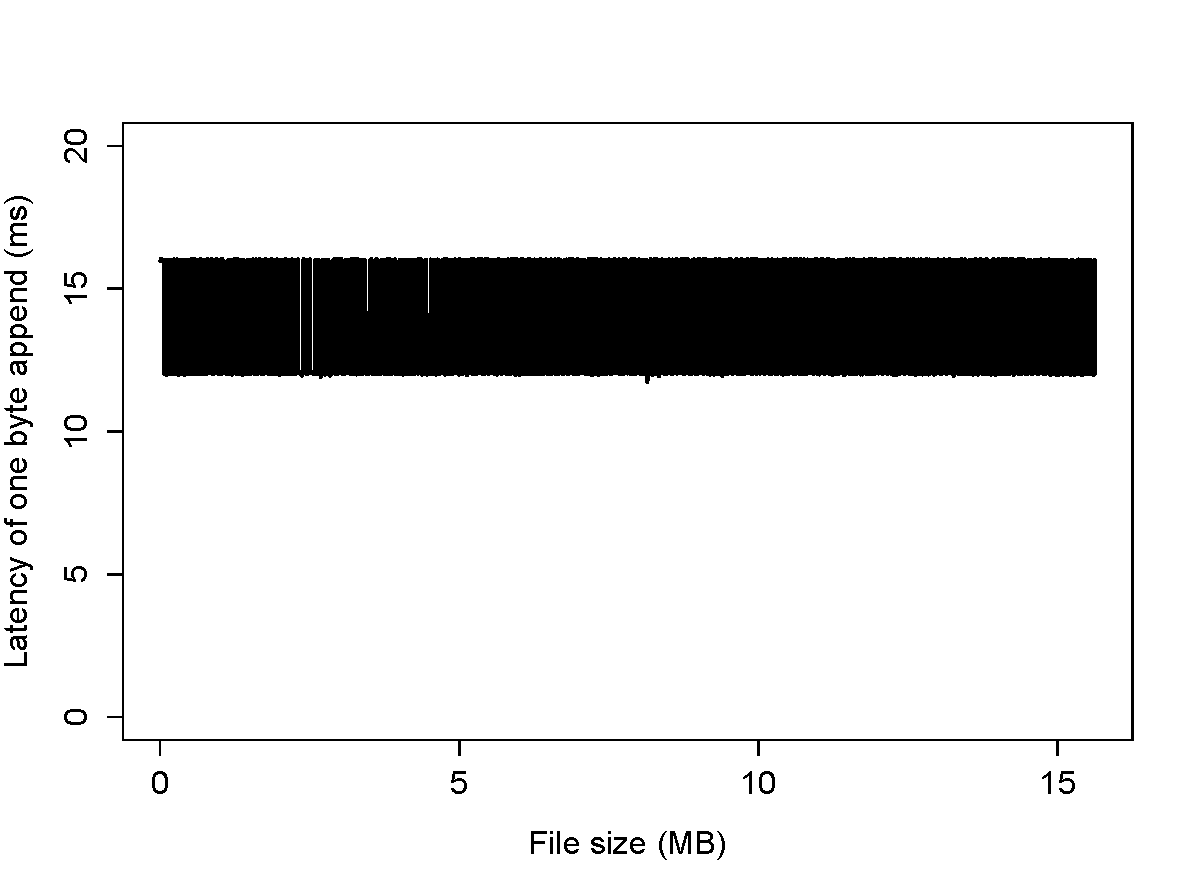
\includegraphics[width=1\textwidth]{./figures/p4_host.pdf}
		\caption{Host}
		\label{fig:p4host}
    \end{subfigure}
    \begin{subfigure}[b]{0.5\textwidth}
		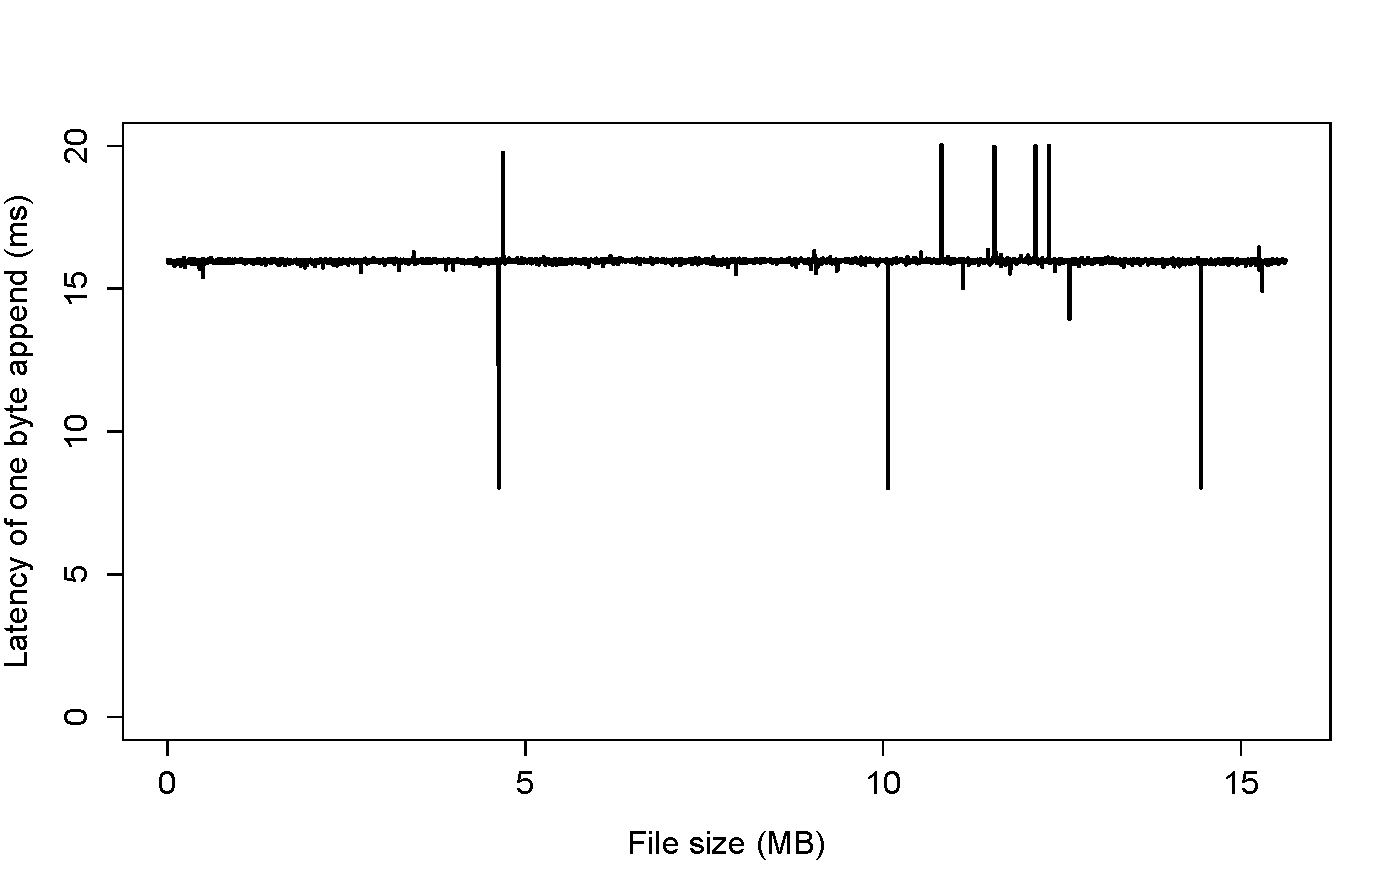
\includegraphics[width=1\textwidth]{./figures/p4_vm.pdf}
		\caption{Virtual machine}
		\label{fig:p4vm}
    \end{subfigure}
	\caption{Latency of one-byte append for varying file sizes. Horizontal axis shows existing file size and vertical axis shows latency of appending one byte to that file.}
	\label{fig:p4}
\end{figure}
